\documentclass{article}
\usepackage[utf8]{inputenc}
\usepackage{amsmath}
\usepackage{listings}
\usepackage{color}
\usepackage{graphicx}
\usepackage[margin=1in]{geometry}
\usepackage{hyperref}
\usepackage{gensymb}
\graphicspath{ {} }

\definecolor{dkgreen}{rgb}{0,0.6,0}
\definecolor{gray}{rgb}{0.5,0.5,0.5}
\definecolor{mauve}{rgb}{0.58,0,0.82}

\lstset{frame=tb,
  language=vhdl,
  aboveskip=3mm,
  belowskip=3mm,
  showstringspaces=false,
  columns=flexible,
  basicstyle={\small\ttfamily},
  numbers=none,
  numberstyle=\tiny\color{gray},
  keywordstyle=\color{blue},
  commentstyle=\color{dkgreen},
  stringstyle=\color{mauve},
  breaklines=true,
  breakatwhitespace=true,
  tabsize=2
}

\title{\textbf{FPGA Temperature Regulation using PID Control in VHDL \\ ECE 4401, Final Project}}
\author{David Paquette}
\date{\today}

\begin{document}

\maketitle

\tableofcontents{}
\newpage
\section{Objective}
Design and build a system to regulate the on board temperature of an FPGA using PID control in VHDL. The desired temperature must be user selectable during system operation. The desired temperature, current temperature and current fan speed must be displayed on an external display. The current temperature and current fan speed must also collected on an external computer.

\section{Introduction}
\subsection{High Level Overview}
The FPGA development board being used is the Nexys 4 DDR Artix-7. This platform contains a built in temperature sensor and push-button pad, used for reading the onboard FPGA temperature and setting the disred temperature, respectively. To cool the FPGA, a DC computer fan is used, specifically the Asus K52F. To modulate the speed of the fan PWM control is used. Any standard VGA display can be used, the FPGA development board has a standard VGA port built in. The FPGA board can also communicate over UART serial using the built in micro-usb connector, this is used to send fan and temperature data to an external computer. An overview of the components used can be seen in figure 1.
\begin{center}
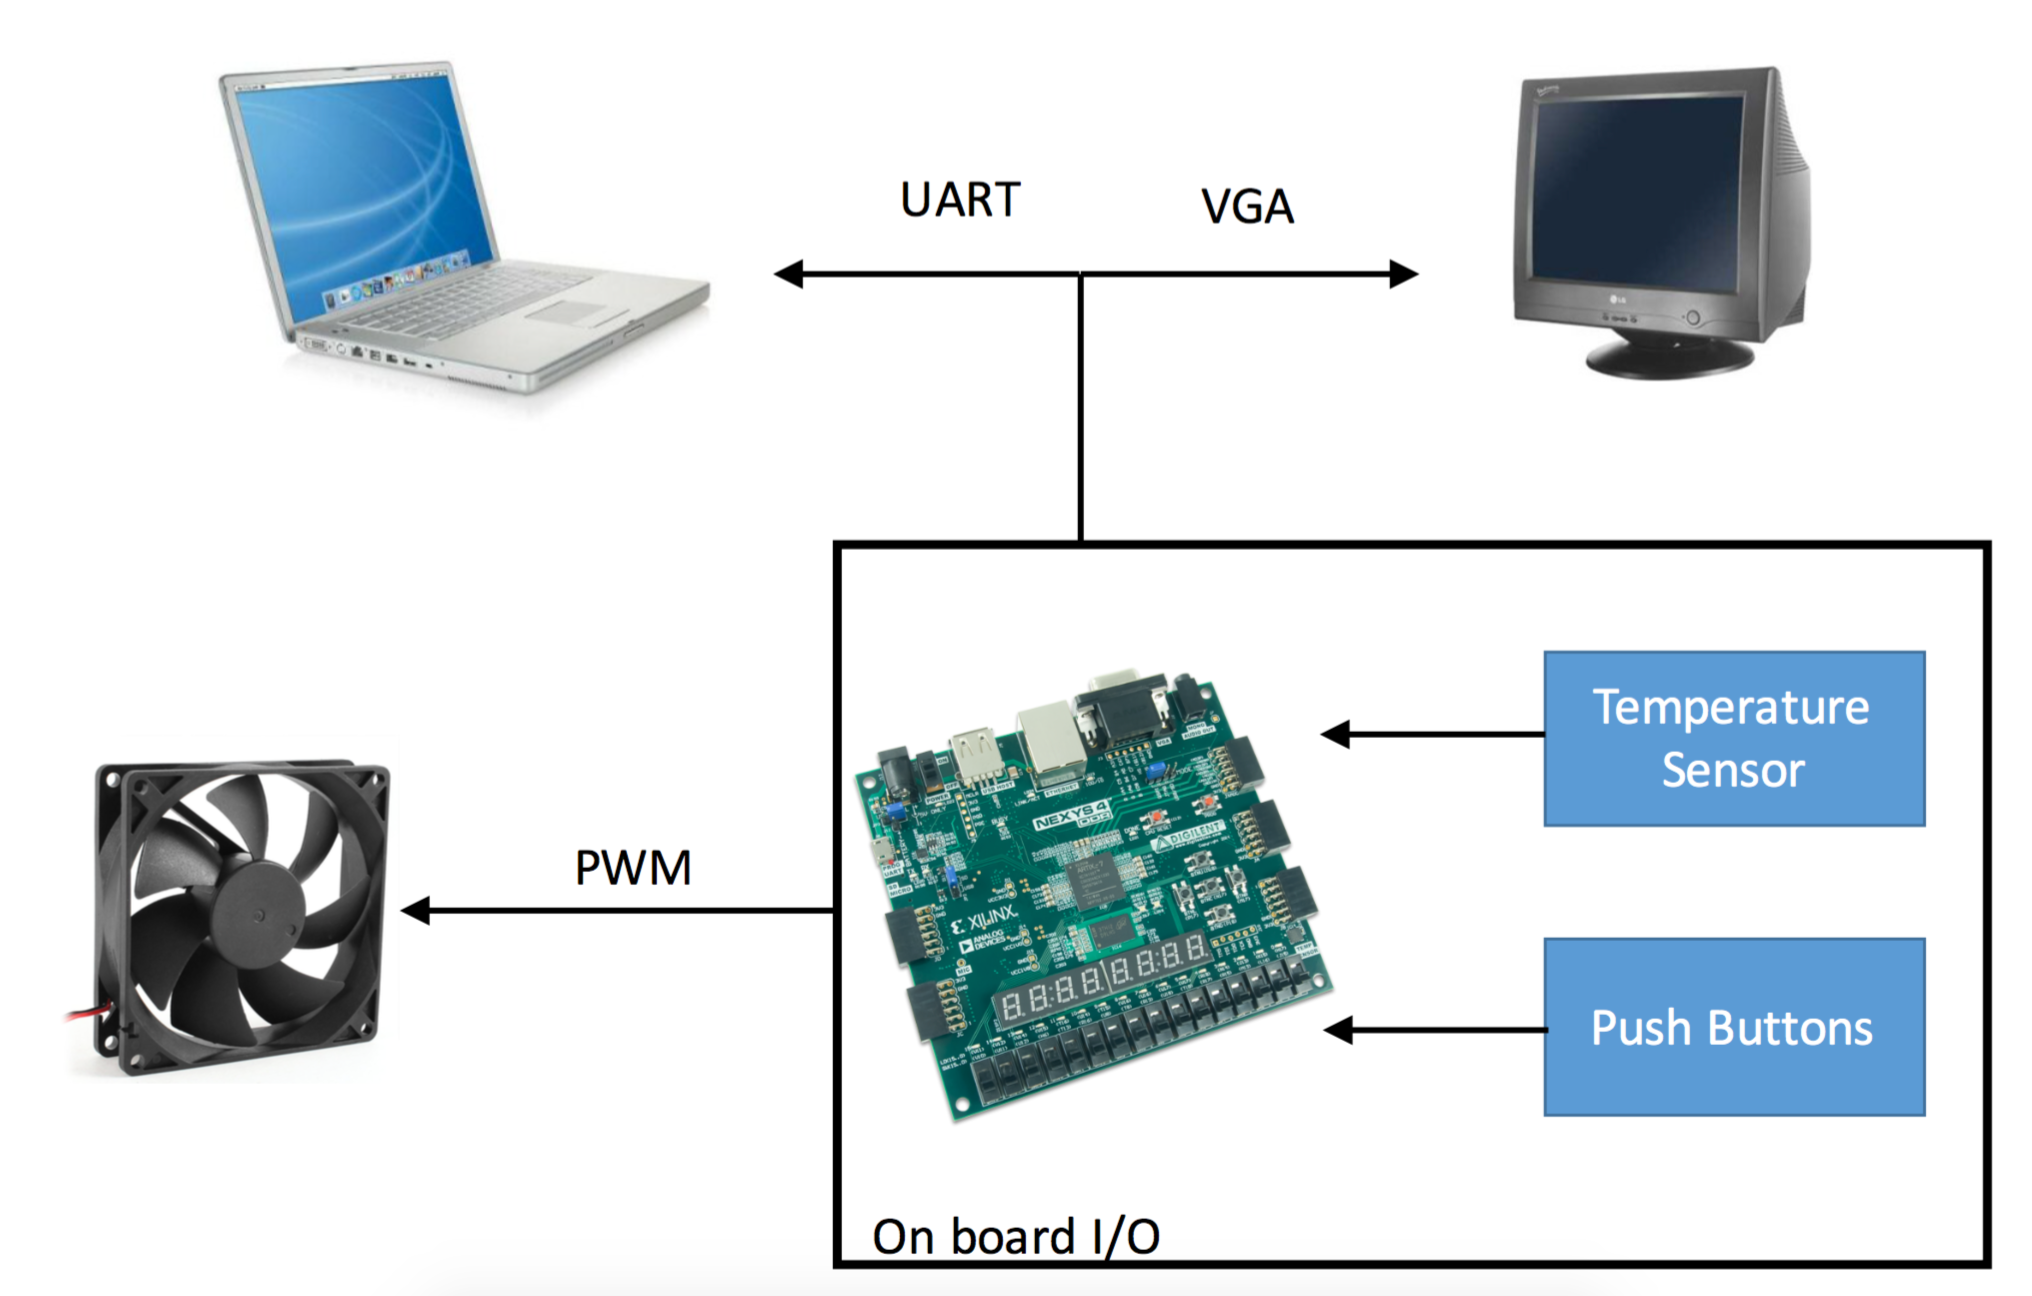
\includegraphics[scale=.4]{images/Overview}\\
\textbf{FIG 1.} High level overview of the system components.\\
\end{center}
\subsection{VHDL Project Overview}
Figure 2 shows an overview of the various VHDL components used in this project. The main modules that were developed for this project were $SetPointControl
$, $PIDController$, $TemperatureSensor$, $PWMInterface$, $Decimal2ASCII$ and $Values2Serial$. The remaining components were orignally written for use in other labs but were reused here. The only entity not developed in this course was the $UART$ component. This library was found online in order to speed up the the development of serial data capture, the original source can be seen in [1]. The three highest level components were instantiated in the top level coponents $TemperatureControlProject$.
\begin{center}
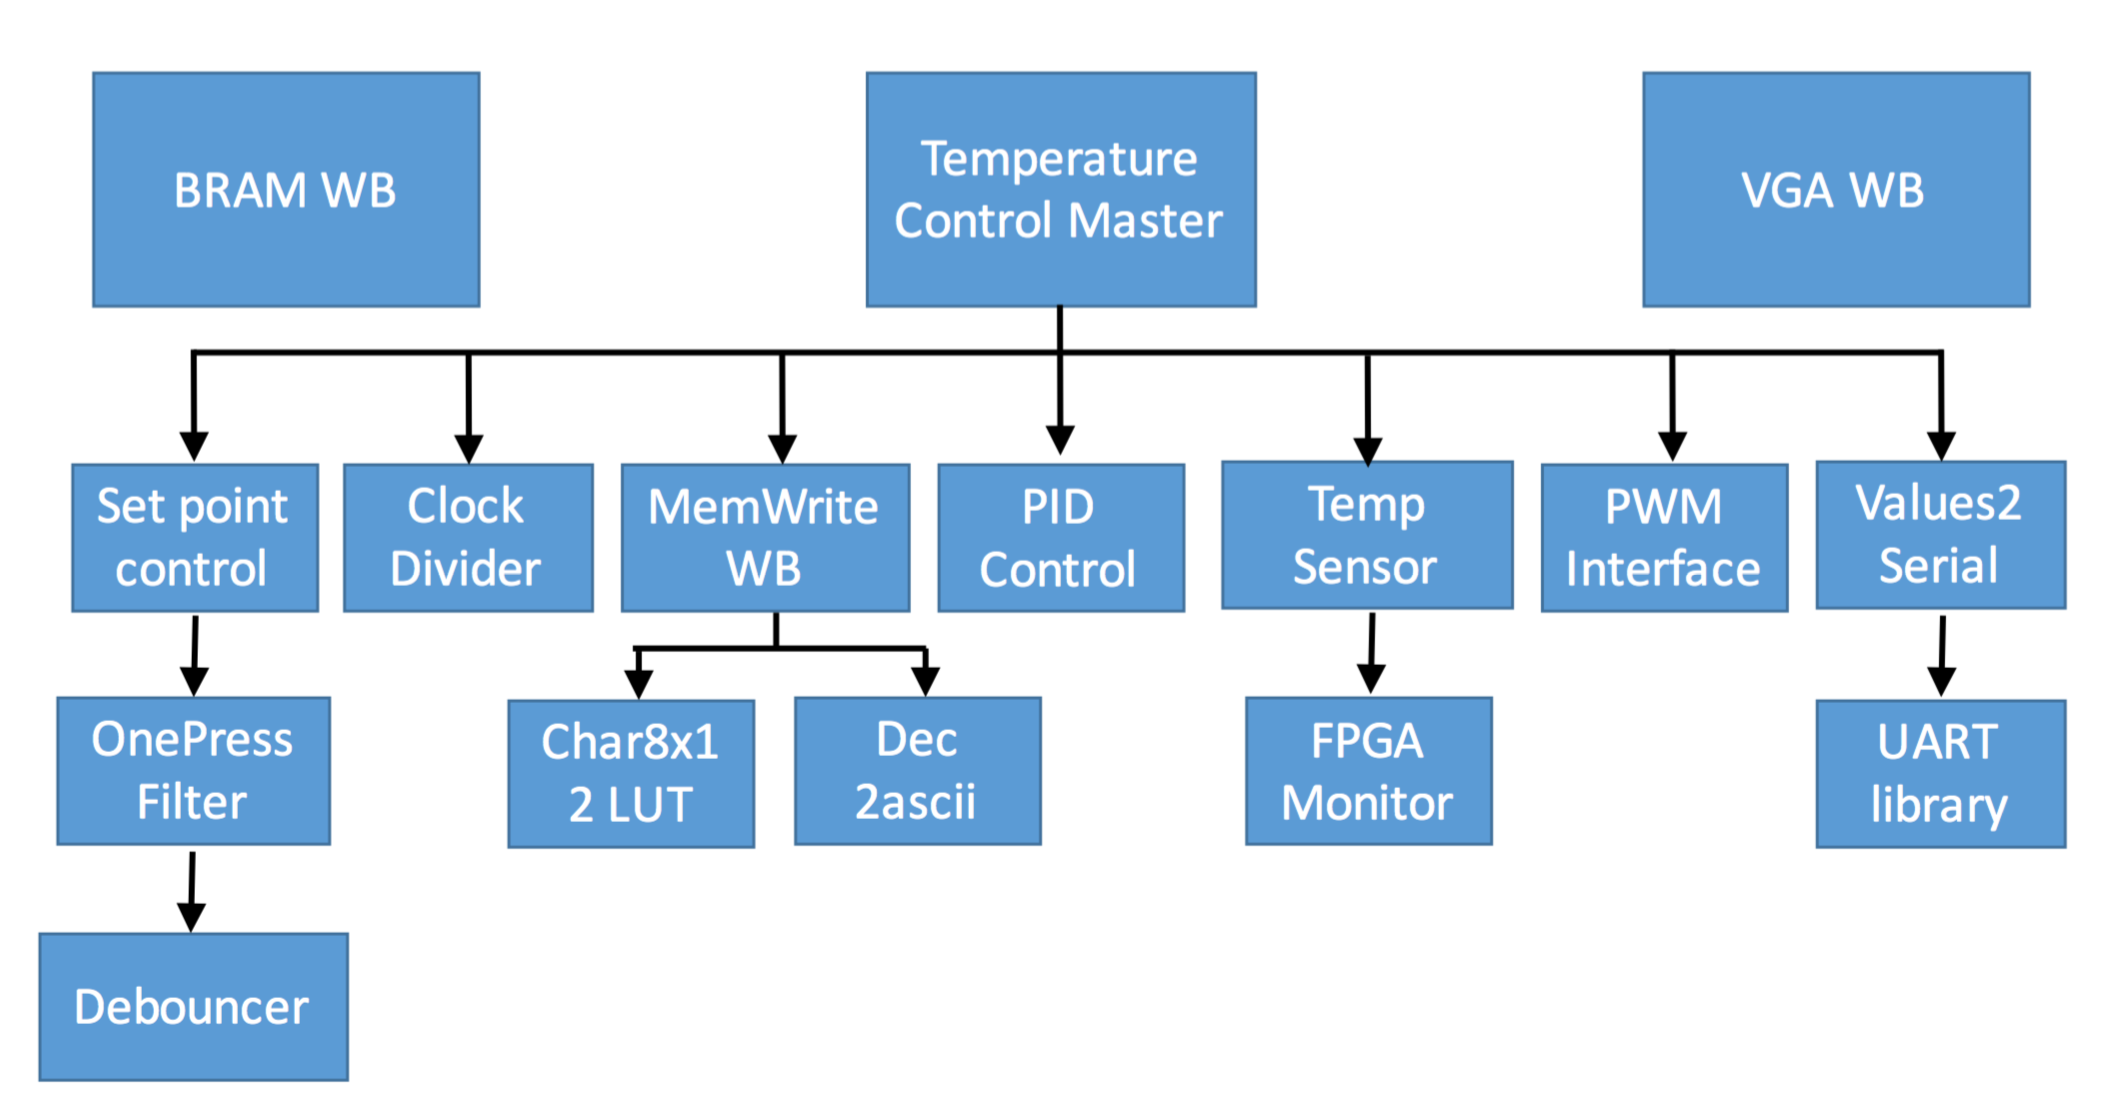
\includegraphics[scale=.35]{images/vhdl_arch}\\
\textbf{FIG 2.} High level VHDL component hierarchy.\\
\end{center}
 
\begin{center}
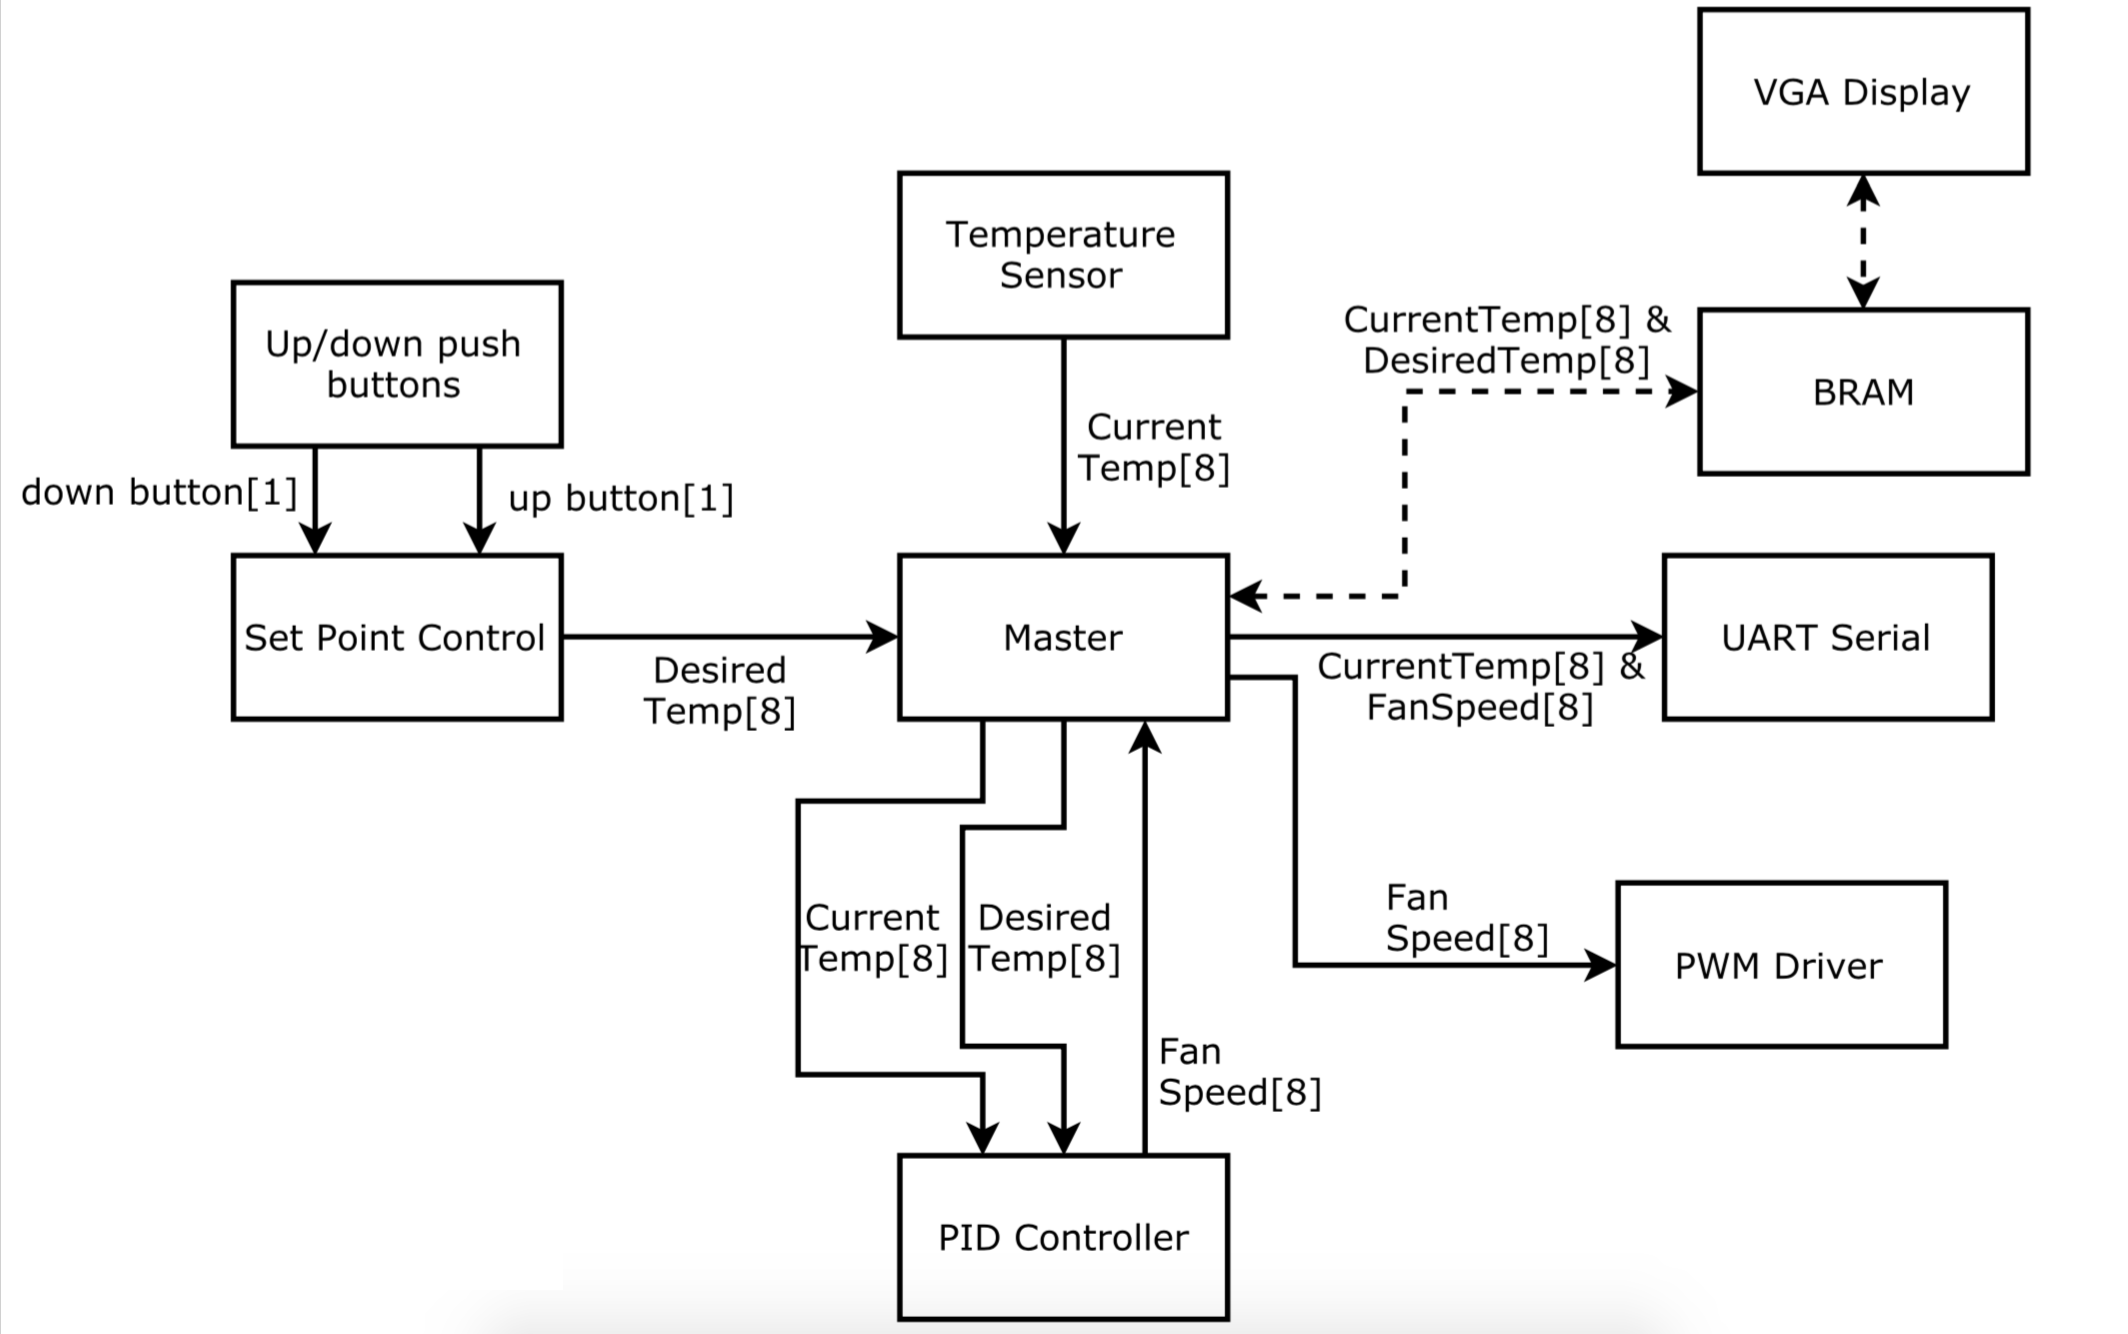
\includegraphics[scale=.4]{images/internalFlow}\\
\textbf{FIG 3.} Main component data path (Wishbone signals are shown as dotted lines).\\
\end{center}

Figure 3 shows the data path of the main components. The $Master$ component contains instantiations of $SetPointControl$, $PIDController$, $PWMDriver$, $TemperatureSensor$ and $UARTSerial$. I decided against making these specific components communicate over the wishbone bus due to the uncetain data send/retrival time that is introduced when communicating over a central bus. Because digital PID control must be normalized over a constant sampling rate, introducing unknown wait cycles did not seem like a good design choice. It may seem odd that I have the VGA controller communicating over the Wishbone bus but not the UART serial communication. This is because during development I was using the serial connection to collect data for the use of system identification and, once again, I did not want to introduce any unnesessary uncertainites into the data. Because the VGA display is just for the user, and is not a system critical component, any delays introduced by the bus wouldn't be an issue.

\section{Temperature Sensor Module}
The temperature sensor used was included on the FPGA development board. The sensor is phycially located on the FPGA. Xilinx provided documentation on how to read and interpret the data from the sensor [2]. Xilinx also provided a VHDL module, $FPGAMonitor$, for returning the ADC(analog-digital converter) code from the on board temperature sensor. The ADC code then needs to be transformed to a meaningful temperature unit, in this project celcius is used. The equation for transforming the ADC code is
\begin{align*}
Temp(\degree C) &= \frac{(ADCode)503.975}{4096}-273.15
\end{align*}
Derived from
\begin{align*}
Voltage &= 10\frac{kT}{q}ln(10)
\end{align*}
Where $k$ is Boltzmann's constant, $T$ is temperature in kelvin and q is the charge on an electron. The analog voltage is sampled by the 12-bit ADCX to produce an ADC code.
 This equation is implemented in the $TemperatureSensorModule$ component. The ADC code is returned in a 12-bit signal, 8-bits for integer values and 4 for decimal. For the sake of simplicity, I will only be using the 8-bits for integer values, which means the accuracy is in $1 \degree$C increments.
\begin{center}
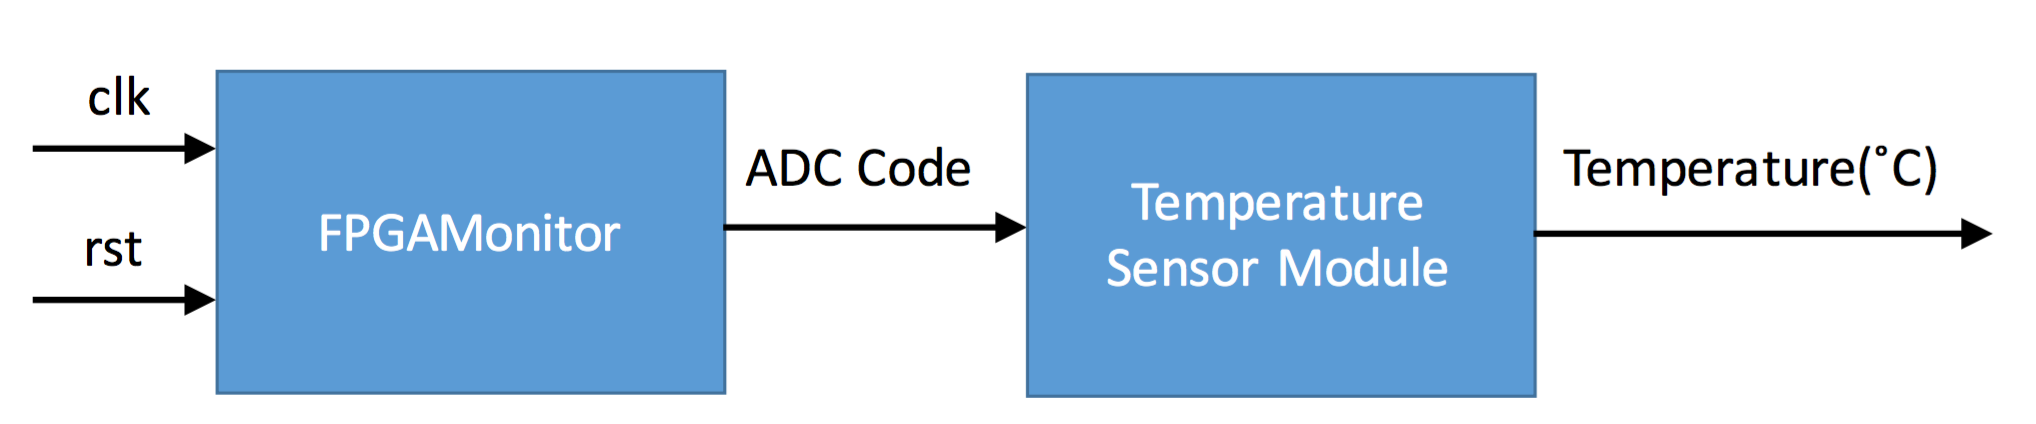
\includegraphics[scale=.5]{images/sensorM}\\
\textbf{FIG 6.} Block diagram of decoding sensor data.\\
\end{center}
\section{Desired Temperature Control Module}
\begin{center}
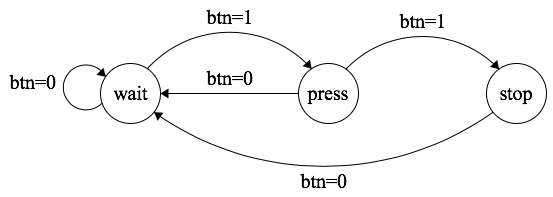
\includegraphics[scale=.5]{images/nopressMachine}\\
\textbf{FIG 7.} State machine describing the One Press Filter.\\
\end{center}
\section{DC Motor Control Module}
\begin{center}
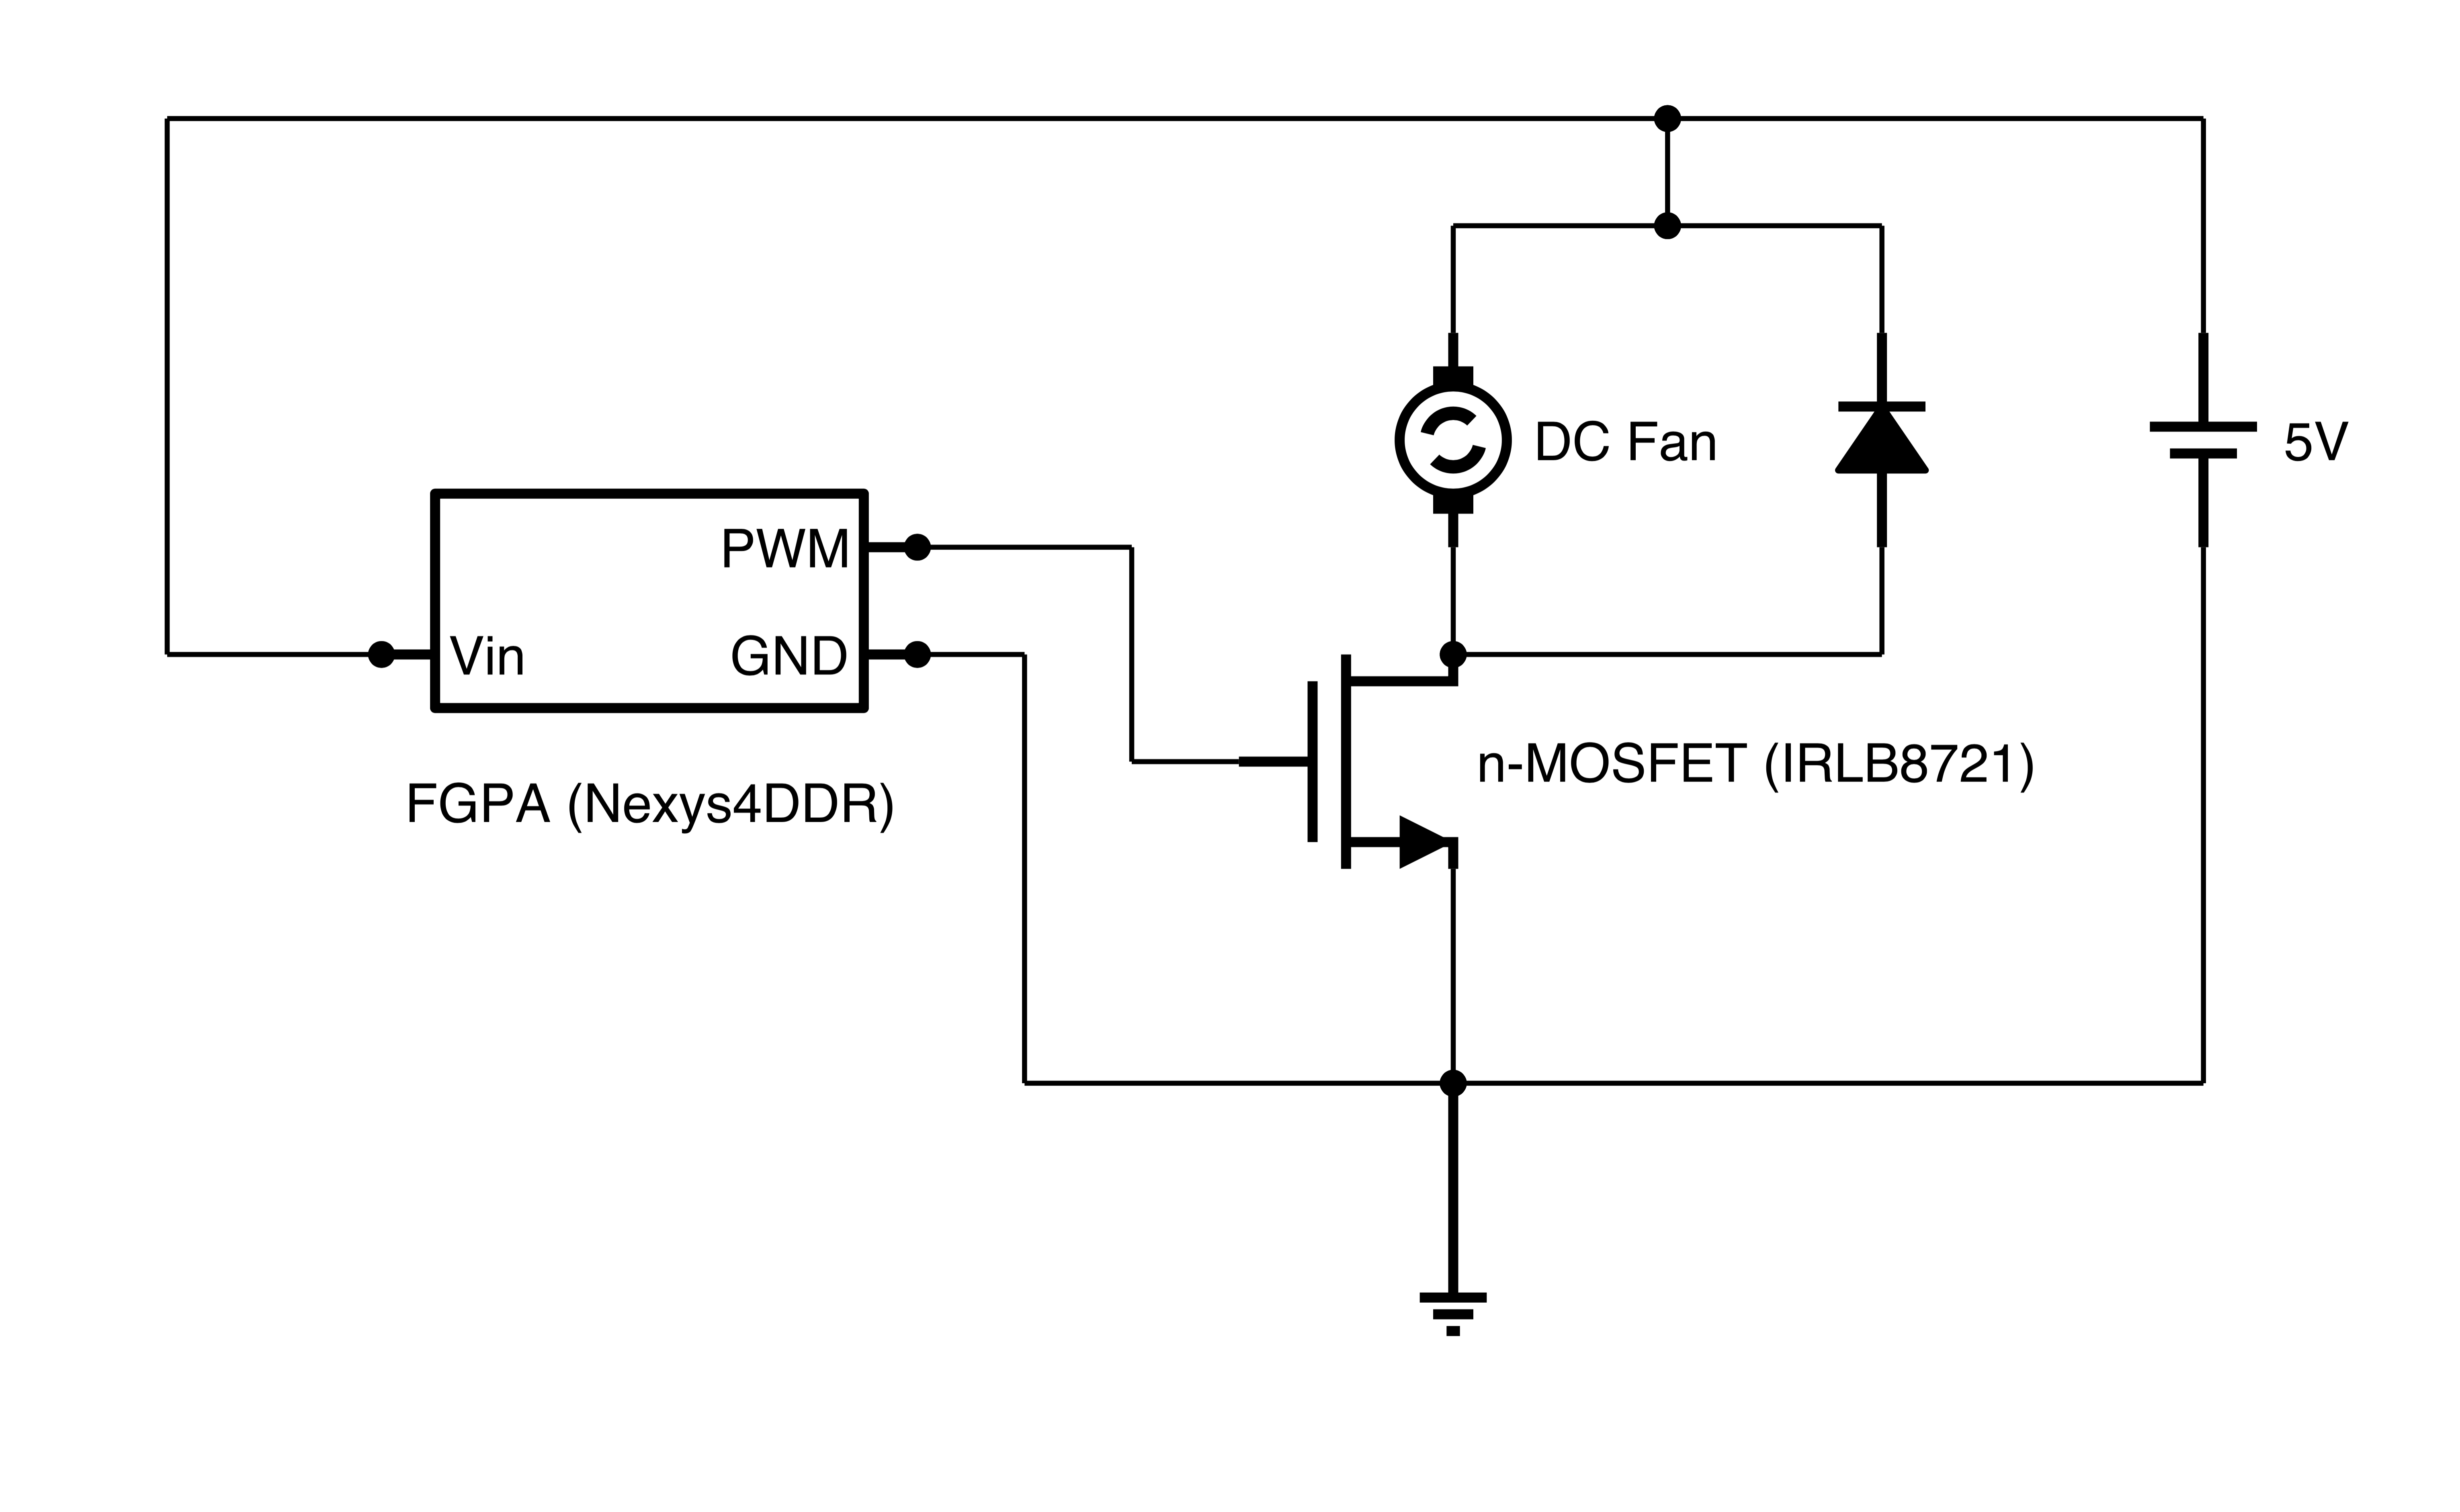
\includegraphics[scale=.5]{images/pwmSchematic-nowords}\\
\textbf{FIG 6.} 3.3V to 5V DC PWM Motor Driver Schematic.\\
\end{center}
\section{UART Serial Communication Module}
\section{VGA BRAM Display Module}
\section{Digital PID Control Module}
\subsection{Discrete PID Control Background}
\begin{align*}
e[k] &= r[k]-y[k]\\
f[k+1] &= K_pe[k]+K_i\sum e[k]T_s + K_d\dfrac{e[k]-e[k-1]}{T_s}\\
T_s&=0.01 s
\end{align*}
The below code sample is the VHDL implementation of the discrete PID controller shown in the equations above.
\begin{lstlisting}
elsif(samplingRateClock'event and samplingRateClock='1') then
			error := (setpoint - sensorFeedbackValue); --compute new error e[k]
			errorSum	:= errorSum + error; --continually compute discrete integral
			if(errorSum > 10000) then --integral wind up check
				errorSum := 10000;
			elsif(errorSum < -10000) then
				errorSum := -10000;
			end if;
			errorChange := error - previousError; --compute discrete derivative
			output := (kp*error + ki*errorSum + kd*errorChange)/100; --compute and scale output
			previousError := error; --save error for use in next iteration for discrete derivative
			if(output>100) then --saturate sensor if needed
				output := 100;
			elsif(output<0)then
				output:=0;
			end if;
			controllerOutput<= output;
	end if;
\end{lstlisting}
\subsection{System Identification}
 \begin{align*}
\boldsymbol{x}[k+1] &= \boldsymbol{A}\boldsymbol{x}[k] + \boldsymbol{B}(\delta[k]-f[k])\\
\boldsymbol{y}[k] &= \boldsymbol{C}\boldsymbol{x}[k]
\end{align*}
\begin{align*}
  \boldsymbol{x}[k+1] &= \begin{bmatrix}
	1 & 0.001 & 0 & 0\\
	0 & 1 & -0.00196 & 0\\
	0 & 0 & 1 &0.001 \\
	0 & 0 & 0.02352 & 1
\end{bmatrix}\boldsymbol{x}[k]+\begin{bmatrix} 0 \\ 0.002 \\ 0 \\ -0.004\end{bmatrix}u[k]\\\\
\boldsymbol{y}[k] &= \begin{bmatrix}
	1 & 0 & 0 & 0\\
	0 & 0 & 1 & 0\\
\end{bmatrix}\boldsymbol{x}[k]
\end{align*}
\subsection{Digital PID Control System Design}
\begin{center}
$K_p=545$	$K_i=150$	$K_d=22$
\end{center}
\section{Temperature Sensor Module}

\section{References}

[1] \url{http://bytebash.com/2011/10/rs232-uart-vhdl} \newline
[2] \url{http://www.xilinx.com/support/documentation/user_guides/ug480_7Series_XADC.pdf}, page 23

\section{Appendix}
1. VHDL implementation of main components.
\end{document}

